\documentclass[10pt]{beamer}
\usepackage[utf8]{inputenc}
\usepackage[spanish]{babel}
\usepackage{amsmath}
\usepackage{amsfonts}
\usepackage{amssymb}
\usepackage{graphicx}
\usepackage{lipsum}
\usepackage{ragged2e}
\usepackage{hyperref} 
\usepackage{float}
\usepackage{tikz}
\usepackage{url}
\usepackage{subcaption}
\usepackage[labelformat=empty]{caption}

\usetheme{Madrid}
\newcommand{\celda}[1]{
	\begin{minipage}{2.5cm}
		\vspace{5mm}
		#1
		\vspace{5mm}
	\end{minipage}
}

\author[Aarón F. Alberca]{Aarón Flores Alberca}
\title[Deep Reinforcement Learning]{Introducción al Deep Reinforcement Learning }
\date{\today} 
\subtitle{Bases teóricas y algoritmos}
% \logo{
\includegraphics[scale=0.0375]{LOGOUNI.pdf}}
\institute[UNI]{
	Universidad Nacional de Ingeniería. Facultad de Ciencias. \\Escuela Profesional de Ciencia de la Computación
}

\AtBeginSection[]
{
	\begin{frame}<beamer>{Contenido}
		\tableofcontents[currentsection,currentsubsection]
	\end{frame}
}

\begin{document}
	
	\begin{frame}
		\maketitle
	\end{frame}

	\begin{frame}{Contenido}
		\tableofcontents
	\end{frame}
	
	\section{Introducción}
		\begin{frame}{Introducción}
            \small
            Fue en 1913, cuando el psicólogo J. B. Watson de la Universidad Johns Hopkins en Estados Unidos escribió el artículo de estudio 'Psychology as the behaviorist views it' en el que, influenciado por la filosfía naturalista de Darwin así como por el trabajo del fisiólogo Iván Pávlov, se abogó por un estudio objetivo de la conducta en los humanos. Esta publicación daría pie a la corriente psicológica del conductismo, la cual se encargaría de estudiar al ser humano a través de estimulos y respuestas del ambiente. Muchos darían críticas a dicha corriente por exentar a sus participantes de una voluntad propia o subconsciente, sino volverlos receptores pasivos del entorno que los rodea.

            \vspace{0.3cm}
            
            \begin{figure}
                \begin{subfigure}[c]{0.4\textwidth}
                    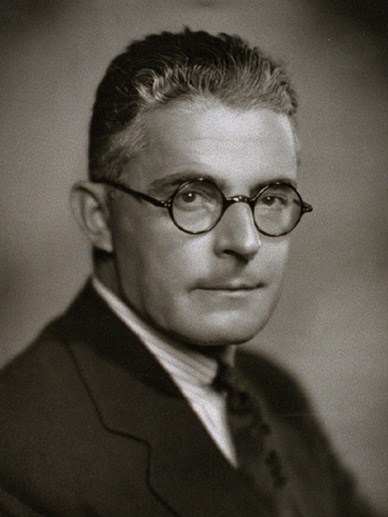
\includegraphics[width=0.5\textwidth]{john-b-watson.jpg}
                    \centering
                    \caption{John B. Watson: Padre del conductismo}
                \end{subfigure}
                \begin{subfigure}[c]{0.4\textwidth}
                    \centering
                    
\includegraphics[width=1\textwidth]{conductismo-social-wide.jpg}
                    \centering
                    \caption{El conductismo estudia el comportamiento observable a través del condicionamiento}
                \end{subfigure}
            \end{figure}

		\end{frame}

        \begin{frame}{Introducción (cont.)}
            Si bien las críticas contra el conductismo fueron acertadas en ciertos aspectos, las matemáticas y las ciencias de la computación encontraron en ella una oportunidad para el desarrollo de un pseudo-aprendizaje en los computadores apartir de la interacción entre un agente y un entorno asignado, llamado hoy en día como Reinforcement Learning o Aprendizaje por refuerzo.

            \vspace{0.5 cm}
            
            El siguiente beamer tiene como objetivo dar a conocer parte de las bases teóricas de dicha rama de la inteligencia artificial, así como explicar su combinación con el Deep Learning para generar el Deep Reinforcement Learning. Por último dar un pequeño ejemplo mostrando un ejemplo con el juego Sonic The Hedgehog para Sega Génesis.
        \end{frame}
        
	\section{Marco teórico}
		\begin{frame}{MDP: Markov Decision Process}
            Los procesos de decisión de Markov o MDP son una formalización matemática al concepto de secuencia de decisiones en una dinámica agente-entorno hacia la completitud de un objetivo. Podemos definir al entorno como todo lo externo a lo que un agente tiene acceso a interactuar y a tener conocimiento, mientras que un agente es aquel que realiza y aprende apartir de realizar acciones que afectan a su entorno haciéndolo cambiar.

            \begin{figure}
                \centering
                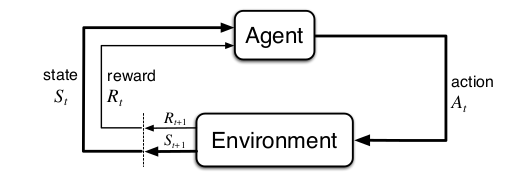
\includegraphics[width=0.8\linewidth]{rl-dynamics.png}
                \caption{La dinámica agente-entorno en un proceso de decisión de Markov}
                \label{fig:enter-label}
            \end{figure}
            
		\end{frame}

        \begin{frame}{MDP: Markov Decision Process (cont.)}
            Podemos definir a un MDP como una serie discreta temporal de pasos $t = 0, 1, 2, \dots$, con la que se recibe una interpretación del estado del entorno inicial $S_t \in \mathcal{S}$ y en base a ella se realiza una acción correspondiente $A_t \in \mathcal{A}(s)$. Posterior a dicho tiempo $t$ se recibe una recompensa $R_{t+1} \in \mathcal{R} \subset \mathbf{R}$ y se regresa a un nuevo estado $S_{t+1} \in \mathcal{S}$. \\
            \vspace{0.3cm}
            Con esto establecemos una secuencia denominada como trayectoria:
            \[
            S_0, A_0, R_1, S_1, A_1, R_2, S_2, A_2, R_3, S_3, \dots
            \]
            
            Es en base a esta secuencia de variables aleatorias que definimos la probabilidad de que haya valores específicos en dicho tiempo dependiendo de una acción y un estado establecidos:
            \[
            p\left( s', r | s, a\right) = \mathrm{P}(S_t = s', R_t = r | S_{t-1} = s, A_{t-1} = a)
            \]
            Para todo $s', s \in \mathcal{S} \wedge r \in \mathcal{R} \wedge a \in \mathcal{A}(s) $
        \end{frame}

        \begin{frame}{MDP: Markov Decision Process (cont.)}
            Lo que quiere declarar la probabilidad definida anteriormente es que la probabilidad conjunta de un estado próximo y su respectiva recompensa dependen del estado y la acción anterior inmediata. (Propiedad implícita de Markov).\\
            \vspace{0.3cm}
            En base a esta probabilidad definida podemos establecer nuevos valores útiles:
           
            \begin{itemize}
                \item Probabilidad de llegar a un estado dado un dado un estado y una acción.
                \[
                p(s'|s,a) = \mathrm{P}(S_t = s' | S_{t-1}=s, A_{t-1} = a) = \sum_{r \in \mathcal{R}} p(s',r | s,a)
                \]
                \item Probabilidad de un recompensa dado un estado y una acción: 
                \[
                p(r|s,a) = \mathrm{P}(R_t = r | S_{t-1}=s, A_{t-1} = a) = \sum_{s' \in \mathcal{S}} p(s',r | s,a)
                \]
            \end{itemize}
        \end{frame}

        \begin{frame}{MDP: Markov Decision Process (cont.)}
            \begin{itemize}
                \item Esperanza de la recompensa dados un estado y una acción:
                \[
                r(s,a) =\mathrm{E}[R_t | S_{t-1}=s, A_{t-1}=a] = \sum_{r \in \mathcal{R}} r \times p(r|s,a)
                \]
                \[
                = \sum_{r \in \mathcal{R}} r \sum_{s' \in \mathcal{S}} p(s', r | s, a)
                \]
                \item Esperanza de la recompensa dados un estado, una acción y el estado próximo:
                \[
                r(s, a, s') = \mathrm{E}[R_t | S_{t-1} = s, A_{t-1} = a, S_t = s'] = \sum_{r \in \mathcal{R}} r \times p(r | s', a, s)
                \]
                \[
                = \sum_{r \in \mathcal{R}} r \frac{p(s', r | s, a)}{p(s' |s,a)} = \frac{\sum_{r \in \mathcal{R}}r \times p(s',r | s,a)}{\sum_{r \in \mathcal{R}} p(s',r|s,a)}
                \]
            \end{itemize}
        \end{frame}
        
		\begin{frame}{Función de retorno}
			Se plantea el hecho de un 'aprendizaje' a partir de una retroalimentación de parte del entorno causado por las acciones del agente; sin 
			embargo aún no hemos definido matemáticamente una recompensa total como producto de una trayectoria, por lo que veamos la siguiente conceptualización:
			
			\[
			G_t = R_{t+1} + \gamma R_{t+2} + \gamma^2 R_{t+3} + \dots + \gamma^{T-1} R_{T} = \sum_{k=t+1}^T \gamma^{k-t-1}R_k
			\]

			De donde $\gamma$ representa un factor de descuento (discount rate) lo que permite dar una cuantificación de que tan valiosas son las recompensas a 
			largo plazo con respecto a las de corto plazo y $T$ es el número de pasos que contiene la trayectoria involucrada. \\
			Este acercamiento permite unificar dos 
			posibles acercamientos al concepto de una trayectoria como episódica (hasta cumplir cierto obejtivo) o continua (sin término).
		\end{frame}

		\begin{frame}{Propiedad de retorno}
			Al analizar con detenimiento nuestra función de recompensa total nos percatamos de lo siguiente:

			\[
			\begin{aligned}
				G_t &= R_{t+1} + \gamma R_{t+2} + \gamma^2 R_{t+3} + \dots + \gamma^{T-t-1} R_{T} \\
				G_t &= R_{t+1} + \gamma \left( R_{t+2} + \gamma R_{t+3} + \dots + \gamma^{T-t-2} R_{T} \right) \\
				G_t &= R_{t+1} + \gamma \left( \sum_{k=t+2}^T \gamma^{k-t-2} R_k \right) \\
				G_t &= R_{t+1} + \gamma G_{t+1}
			\end{aligned}
			\]

			Es así como logramos obtener una recursión representada la recompensa total de un estado futuro como $G_{t+1}$, esta definición nos será de 
			utilidad para la siguiente sección.
		\end{frame}

		\begin{frame}{Políticas y funciones}
			Definimos a una política como un mapeo de los estados a las probabilidades de seleccionar las acciones disponibles en estas; matemáticamente podríamos definir 
			la siguiente expresión sobre lo que se refiere a una política:

			\[
			\pi(a | s) = P(A_t = a | S_t = s)
			\]

			El objetivo final de todo algoritmo de Reinforcement Learning es lograr una definición de una política adecuada adaptada a un objetivo en específico 
			para ayudar al agente a completarlo eficientemente. Esta nueva función nos permite redefinir algunos conceptos anteriores, para lo cual podremos hacer uso de ciertas propiedades
			de las variables aleatorias y la estadística:

			\begin{itemize}
				\item \textbf{Regla de la cadena de probabilidades condicionales:} Derivado de la ley de Bayes podemos factorizar una probabilidad conjunta de algun vector de variables aleatorias $\mathrm{X} = X_1, X_2, \dots X_n$ a una productoria.
				\[
				P(X_1, X_2, X_3, \dots, X_n) = \prod_{i=1}^n P \left( X_i | \bigcap_{j=1}^{i-1} X_j \right)
				\]
			\end{itemize}
		\end{frame}

		\begin{frame}{Políticas y funciones (cont.)}
			\begin{itemize}
				\item \textbf{Ley de las esperanzas totales:} Se nos es permitido la obtención de la esperanza de una variable aleatoria $X$ al calcular la esperanza de la esperanza de otra variable aleatoria $Y$ como $Y|X$
				\[
				E[X] = E[E[X|Y]] = \sum_i E[X | Y_i] P(Y_i)
				\]
			\end{itemize}

			Con aquello podemos obtener la siguiente fórmula para la esperanza de una recompensa $R_{t+1}$ dado un estado inicial $S_t$ siguiendo una política estocástica $\pi$
			\[
			\begin{aligned}
				E[R_{t+1} | S_t = s, A_t = a] &= r(s, a) = \sum_{s' \in \mathcal{S}} p(s' | a, s) \times r(s, a, s')  \\
				E[R_{t+1} | S_t = s] &= \sum_{a \in \mathcal{A}(s)} \pi(a | s) \times r(s, a) \\
				&= \sum_{a \in \mathcal{A}(s)} \pi(a | s) \sum_{s' \in \mathcal{S}} p(s' | a, s) \times r(s, a, s') \\
				&= \sum_{a \in \mathcal{A}(s)} \pi(a | s) \sum_{s' \in \mathcal{S}} \sum_{r \in \mathcal{R}} r \times p(s',r | s,a)
			\end{aligned}
			\]
		\end{frame}

		\begin{frame}{Políticas y funciones (cont.)}
			Ahora que contamos con una definición mas adecuada de una política, podemos pasar a ciertas funciones que también nos permiten determinar adecuadamente estimar las recompensas
			no solo de un estado en específico sino que de la recompensa total de una trayectoria, mediante las funciones de valor $V_{\pi}(s)$ y la función acción-valor $Q_{\pi}(s, a)$.
			Son definidas matemáticamente de la siguiente forma:

			\begin{itemize}
				\item \textbf{Función valor:}
				\[
				V_{\pi}(s) = E_{\pi}\left[G_t | S_t = s\right] 
				\]
				\item \textbf{Función acción-valor:}
				\[
				Q_{\pi}(s, a) = E_{\pi}\left[G_t | S_t = s, A_t = a\right]
				\]
			\end{itemize}

			De donde se cumple la siguiente propiedad:
			\[
			V_{\pi}(s) = \sum_{a \in \mathcal{A}(s)} \pi(a | s) E_{\pi}\left[G_t | S_t = s, A_t = a\right] = \sum_{a \in \mathcal{A}(s)} \pi(a | s) Q_{\pi}(s, a)
			\]

			Afortunadamente, podemos desglosar muchísimo más de dichas funciones a partir de la función recursiva de $G_t$ para definir las funciones de Bellman
		\end{frame}

		\begin{frame}{Políticas y funciones (cont.)}
			Para la función valor tenemos:
			\[
			\begin{aligned}
			V_{\pi}(s) &= E_{\pi}\left[G_t | S_t = s\right] = E_{\pi}\left[R_{t+1} + \gamma G_{t+1} | S_t = s\right] \\	
			&= E_{\pi}\left[R_{t+1} | S_t = s \right] + \gamma E_{\pi}\left[G_{t+1} | S_t=s\right]
			\end{aligned}
			\]
			
			Nos falta el segundo término a completar, ya que el primero lo obtuvimos en una anterior diapositiva:

			\vspace{0.2 cm}

			\resizebox{\textwidth}{!}{
			$E[G_{t+1} | S_t = s, A_t = a] = \sum_{s' \in \mathcal{S}} \sum_{r \in \mathcal{R}} p(s', r | a, s)  E[G_{t+1} | S_t = s, A_t = a, S_{t+1} = s', R_{t+1} = r]$
			}
			
			\vspace{0.2 cm}
			Mediante la propiedad de Markov podemos simplificar la expresión anterior, ya que $G_{t+1}$ solo dependerá del estado $S_{t+1} = s'$

			\[
				\begin{aligned}
					E[G_{t+1} | S_t = s, A_t = a] &= \sum_{s' \in \mathcal{S}} \sum_{r \in \mathcal{R}} p(s', r | a, s)  E[G_{t+1} | S_{t+1} = s'] \\
					E[G_{t+1} | S_t = s] &= \sum_{a \in \mathcal{A}(s)} \pi(a | s) \times E[G_{t+1} | S_t = s, A_t = a]  \\
					&= \sum_{a \in \mathcal{A}(s)} \pi(a | s) \sum_{s' \in \mathcal{S}} \sum_{r \in \mathcal{R}} p(s', r | a, s) E[G_{t+1} | S_{t+1} = s']
				\end{aligned}
			\]
		\end{frame}

		\begin{frame}{Políticas y funciones (cont.)}
			Con todo lo obtenido, podemos redefinir a nuestra función valor de la siguiente forma:
			
			\[
			\begin{aligned}
				V_{\pi}(s) &= E_{\pi}\left[R_{t+1} | S_t = s \right] + \gamma E_{\pi}\left[G_{t+1} | S_t=s\right] \\
				&= \sum_{a \in \mathcal{A}(s)} \pi(a | s) \sum_{s' \in \mathcal{S}} \sum_{r \in \mathcal{R}} p(s', r | a, s) \left(r + \gamma \times E[G_{t+1} | S_{t+1} = s'] \right) \\
				&= \sum_{a \in \mathcal{A}(s)} \pi(a | s) \sum_{s' \in \mathcal{S}} \sum_{r \in \mathcal{R}} p(s', r | a, s) \left(r + \gamma \times V_{\pi}(s') \right)			
			\end{aligned}
			\]

			Así logramos redefinir a nuestra función valor como una recursiva en base a un estado futuro $s'$, con esto nosotros habremos llegado a la ecuación de Bellman para la función valor.
		\end{frame}

		\begin{frame}{Políticas y funciones (cont.)}
			Para la función acción-valor:
			\[
			\begin{aligned}
				Q_{\pi}(s, a) &= E_{\pi}[G_t | S_t = s, A_t = a] = E_{\pi}[R_{t+1} + \gamma G_{t+1} | S_t = s, A_t = a] \\
				&= E_{\pi}[R_{t+1} | S_t = s, A_t = a] + \gamma E_{\pi}[G_{t+1} | S_t = s, A_t = a]
			\end{aligned}
			\]

			Ahora solo para fines de aclaraciones definiremos los términos encontrados en base de lo hallado mediante en las anteriores definiciones matemáticas:

			\[
			\begin{aligned}
				E_{\pi}[R_{t+1} | S_t = s, A_t = a] &= \sum_{s' \in \mathcal{S}} \sum_{r \in \mathcal{R}} r \times p(s', r | s , a) \\
				E_{\pi}[G_{t+1} | S_t = s, A_t = a] &= \sum_{s' \in \mathcal{S}} \sum_{r \in \mathcal{R}} p (s', r | a, s) E[G_{t+1} | S_{t+1} = s'] \\
				&= \sum_{s' \in \mathcal{S}} \sum_{r \in \mathcal{R}} p (s', r | a, s) \sum_{a' \in \mathcal{A}(s')} \pi(a' | s') Q_{\pi}(s', a')
			\end{aligned}
			\]
		\end{frame}

		\begin{frame}{Políticas y funciones (cont.)}
			Finalmente logramos descubrir nuevamente una versión recursiva de la función acción-valor con la siguiente definición:
			\[
			Q_{\pi}(s, a) = \sum_{s' \in \mathcal{S}} \sum_{r \in \mathcal{R}} p(s', r | a, s) (r + \gamma \times \sum_{a' \in A(s')} \pi(a' | s') 	Q_{\pi}(s', a'))
			\]

			Con todo lo conseguido hasta ahora hemos logrado obtener las diferentes ecuaciones de Bellman con respecto a la funciones de valor y acción-valor.
		\end{frame}

		\begin{frame}{Optimización de funciones}
			\small
            El objetivo en Reinforcement Learning es encontrar la política óptima $\pi^*$ que maximice la suma de recompensas totales. Para ello definimos:
            \[
            \pi^* = \arg\max_\pi V_\pi(s) \quad \forall s \in \mathcal{S}
            \]
            Esto implica determinar la función de valor óptima:
            \[
            V^*(s) = \max_\pi V_\pi(s)
            \]
            y la función acción-valor óptima:
            \[
            Q^*(s,a) = \max_\pi Q_\pi(s,a)
            \]

			De las que si tomamos nuestra anterior relación entre las funciones valor y acción-valor, obtenemos lo siguiente:
			\[
			V^*(s) = \max_{a \in \mathcal{A}(s)} Q^*(s, a)
			\]


            Las ecuaciones de Bellman óptimas se expresan como:
            \[
            V^*(s) = \max_{a \in \mathcal{A}(s)} \sum_{s',r} p(s',r|s,a) \left( r + \gamma V^*(s') \right)
            \]
            \[
            Q^*(s,a) = \sum_{s',r} p(s',r|s,a) \left( r + \gamma \max_{a'} Q^*(s',a') \right)
            \]
        \end{frame}
	
	\section{Algoritmos de gradiente de política}
		\begin{frame}{Un nuevo enfoque}
			A pesar de las anteriores explicaciones analizando los conceptos de las funciones valor, acción-valor y política, la determinación de 
			sus versiones óptimas resultan ser demasiado complicados en entornos cuyos estados tienen una representación numérica compleja o presentan
			variables ocultas para el agente dando como consecuencia un costo computacional absurdo.
			\vspace{0.3 cm}
			
			Para resolver este problema, tomamos un nuevo enfoque para el cual no se toman en consideración las funciones de valor y acción-valor, sino que hacemos
			uso de un \textbf{estimador} que permita el cálculo de los valores de la política dado un conjunto de parámetros $\boldsymbol{\theta} \in \mathrm{R}^k$ que representen valores que componen dicho estimador. Así definimos
			el siguiente concepto:
			
			\[
			\pi(a | s, \boldsymbol{\theta}) = P(A_t = a | S_t = s, \boldsymbol{\theta}_t = \boldsymbol{\theta})
			\]

			Con esta pequeña introducción nosotros entramos Deep Reinforcement Learning al usar una red neuronal como dicho \textbf{estimador}, teniendo a nuestros parámetros
			$\boldsymbol{\theta}$ a los pesos de dicha red.
		\end{frame}
		
		\begin{frame}{Algoritmos de gradiente de política}
			Comenzamos definiendo a nuestra función de evaluación de política $J(\boldsymbol{\theta})$ con respecto a los parámetros de dicha política. Usualmente definida de la siguiente forma:
			\[
			J(\boldsymbol{\theta}) = V_{\pi_{\boldsymbol{\theta}}} (s_0) = E_{\pi_{\boldsymbol{\theta}}} \left[G_t | S_t = s_0\right]
			\]

			En base esta, haremos uso del método de gradiente ascendiente para lograr encontrar valores para dichos parámetros que maximizen la recompensa total:

			\[
			\boldsymbol{\theta}_{t+1} = \boldsymbol{\theta}_t + \alpha \widehat{\nabla J(\boldsymbol{\theta}_t)} 
			\]

			Donde $\alpha \in \left[0, 1\right]$ se define como la tasa de aprendizaje y $\widehat{\nabla J(\boldsymbol{\theta}_t)} \in \mathrm{R}^k$ a un estimación estocástica cuyo valor esperado se aproxima
			a la gradiente de la función de evaluación de política con respecto a sus parámetros.
			\vspace{0.3 cm}
			
			Es así como definimos a todos los posibles algoritmos que sigan este esquema de optimización como 'algoritmos de gradiente de política' y si 
			deciden tambien estimar la función valor entonces son llamados 'algoritmos de actor-crítico', donde el denominado actor es quien estima la política
			y el crítico estima la función valor.
		\end{frame}

		\begin{frame}{El teorema de la política de gradiente}
			En comparación con otros métodos, la política de gradiente ofrece una ventaja teórica significativa, ya que es menos susceptible a cambios abruptos, en comparación con otros enfoques
			como $\epsilon$-greedy en el que se pueden experimentar cambios drámaticos ante mínimas modificaciones en sus valores estimados de acción. Es justamente aquello por lo que los métodos de 
			política de gradiente presentan una mayor posibilidad de convergencia que métodos de funciones acción-valor.
			Sin embargo, ¿cómo es que podemos estimar la gradiente de la función de evaluación de política con respecto a su parámetros cuando dicha gradiente depende del efecto \textbf{desconocido} de los cambios
			a la política con la distribución de estados?
			\vspace{0.3 cm}

			Afortunadamente contamos con la respuesta a dicha incertidumbre dentro del teorema de la política de gradiente, la cual indica una expresión analítica a la gradiente solicitada sin ninguna derivación en 
			la distribución de estados y se define como:

			\[
			\nabla J(\boldsymbol{\theta}) \propto \sum_{s \in \mathcal{S}} \mu(s) \sum_{a \in \mathcal{A}(s)} Q_{\pi}(s, a) \nabla \pi(a | s, \boldsymbol{\theta})
			\]
		\end{frame}

		\begin{frame}{Demostración del teorema de la política de gradiente}
			Comenzaremos buscando obtener la gradiente de la función valor en términos de la función acción-valor y para simplificar notación asumiremos que nuestra política ya esta definida por los parámetros $\boldsymbol{\theta}$
			\[
			\begin{aligned}
				\nabla v_{\pi}(s) &= \nabla \left[\sum_a \pi(a | s) Q_\pi (s, a)\right] \\
				&= \sum_a \left[\nabla \pi(a | s) Q_\pi(s,a) + \pi(a | s) \nabla Q_\pi(s, a)\right] \\
				&= \sum_a \left[\nabla \pi(a | s) Q_\pi(s,a) + \pi(a | s) \nabla \left( \sum_{s', r} p(s', r | s, a) (r + \gamma V_\pi(s')) \right)\right] \\
				&= \sum_a \left[\nabla \pi(a | s) Q_\pi(s,a) + \pi(a | s) \left( \sum_{s'} p(s' | s, a) \gamma \nabla V_\pi(s') \right)\right] \\
			\end{aligned}
			\]
		\end{frame}
		
		\begin{frame}{Demostración del teorema de la política de gradiente (cont.)}
			\[
			\begin{aligned}
				&\begin{aligned}
					= \sum_a \Bigg[ \nabla &\pi(a | s) Q_\pi(s,a) + \pi(a | s) \sum_{s'} p(s' | s, a) \\
					&\gamma \sum_{a'} \Big[ \nabla \pi(a' | s') Q_\pi(s',a') + \pi(a' | s') \sum_{s''} p(s'' | s', a') \gamma \nabla V_\pi(s'') \Big] \Bigg] 
				\end{aligned} \\
				&= \sum_{x \in \mathcal{S}} \sum_{k=0}^\infty \gamma^k P(s \rightarrow x, k, \pi) \sum_{a} \nabla \pi(a | x) Q_\pi (x, a)
			\end{aligned}
			\]
			De donde $P(s \rightarrow x, k, \pi)$ resulta ser la probabilidad de transicionar de un estado $s$ a un estado $x$ en $k$ pasos dentro de una política $\pi$. La razón de 
			la última conversión es que al seguir iterando la sumatoria nosotros nos encontramos con repetición de futuros estados en los que abrir paso a una gran múltiplicación interna como la que se muestra en la propiedad anterior para todos los estados posibles.
		\end{frame}

		\begin{frame}{Demostración del teorema de la política de gradiente (cont.)}
			Antes de seguir definamos los siguientes conceptos:

			\begin{itemize}
				\item \textbf{Tiempo dentro de un estado}: Cantidad de veces que se alcanzo un estado $s$ desde un estado inicial $s_0$, podemos expresarlo matemáticamente como:
				\[
				\eta(s) = \sum_{k=0}^\infty \gamma^k P(s_0 \rightarrow s, k, \pi)
				\]
				\item \textbf{Distribución de estados}: Distribución probabilística de los estados alcanzados mediante una política $\pi$, la función asociada a ella nos dice su razón de aparición desde un estado inicial $s_0$
				\[
				\mu(s) = \frac{\eta(s)}{\sum_{s'}\eta(s')}
				\]
			\end{itemize}
		\end{frame}

		\begin{frame}{Demostración del teorema de la política de gradiente (cont.)}
			Ahora continuamos con el presente cálculo obtenido para hallar la gradiente de la función de evaluación de política:
			\[
			\begin{aligned}
				\nabla J (\boldsymbol{\theta}) &= \nabla V_\pi(s_0) \\
				&= \sum_{s \in \mathcal{S}} \left(\sum_{k=0}^\infty \gamma^k P(s_0 \rightarrow s, k, \pi)\right) \sum_{a} \nabla \pi(a | s) Q_\pi (s, a) \\
				&= \sum_{s \in \mathcal{S}} \eta(s) \sum_a \nabla \pi(a | s) Q_\pi(s, a) \\
				&= \sum_{s' \in \mathcal{S}} \eta(s') \sum_{s \in \mathcal{S}} \frac{\eta(s)}{\sum_{s'}\eta(s')} \sum_a \nabla \pi(a | s) Q_\pi(s, a) \\
				&= \sum_{s' \in \mathcal{S}} \eta(s') \sum_{s \in \mathcal{S}} \mu(s) \sum_a \nabla \pi(a | s) Q_\pi(s, a) \\
				&\propto \sum_{s \in \mathcal{S}} \mu(s) \sum_a \nabla \pi(a | s) Q_\pi(s, a) 
			\end{aligned}
			\]
		\end{frame}

		\begin{frame}{Demostración del teorema de la política de gradiente (cont.)}
			Con esta definición somos capaces de poder abstraerla a un concepto de esperanza analizando lo siguiente:
			\[
			\begin{aligned}
				\nabla J(\boldsymbol{\theta}) &\propto \sum_{s \in \mathcal{S}} \mu(s) \sum_a Q_\pi(s, a) \pi(a | s, \boldsymbol{\theta}) \frac{\nabla \pi(a | s, \boldsymbol{\theta})}{\pi(a | s, \boldsymbol{\theta})} \\
				&\propto \sum_{s \in \mathcal{S}} \mu(s) \sum_a Q_\pi(s, a) \pi(a | s, \boldsymbol{\theta}) \nabla \ln(\pi(a | s, \boldsymbol{\theta})) \\
				&\propto E_\pi \left[\sum_a Q_\pi (S_t, a) \pi(a | s, \boldsymbol{\theta}) \nabla \ln(\pi(a | s, \boldsymbol{\theta}))\right] \\
				&\propto E_\pi \left[G_t \nabla \ln(\pi(a | s, \boldsymbol{\theta}))\right]
			\end{aligned}
			\]
		\end{frame}
	
%%	\section{Proximal Policy Optimization - PPO}

%% 	\section{Group Relative Policy Optimization - GRPO}


%\appendix
\section{Referencias}
%\subsection<presentation>*{Referencias}

\begin{frame}{Referencias}
	[1] M. Lehmann, “The Definitive Guide to Policy Gradients in Deep Reinforcement Learning: Theory, Algorithms and Implementations.” Available: \url{https://arxiv.org/abs/2401.13662}
	\vspace{0.3 cm}

	[2] J. Schulman, F. Wolski, P. Dhariwal, A. Radford, and O. Openai, “Proximal Policy Optimization Algorithms,” Aug. 2017. Available: \url{https://arxiv.org/abs/1707.06347}
	\vspace{0.3 cm}

	[3] K. Grolinger, “Reinforcement Learning Algorithms: An Overview and Classification.” Available: \url{https://arxiv.org/abs/2209.14940}
	\vspace{0.3 cm}

	[4] Sutton, R. S., \& Barto, A. G. (2018). Reinforcement learning: An introduction (2nd ed.). The MIT Press. Available: \url{http://incompleteideas.net/book/RLbook2020.pdf}
	\vspace{0.3 cm}

	[5] Shao, Z., Wang, P., Zhu, Q., Xu, R., Song, J., Bi, X., Zhang, H., Zhang, M., Li, Y. K., Wu, Y., \& Guo, D. (2024, 5 febrero). DeepSeekMath: Pushing the Limits of Mathematical Reasoning in Open Language Models. Available: \url{https://arxiv.org/abs/2402.03300}
\end{frame}

\end{document}